% !TEX root = marvin.tex
\section{Experiments}
\subsection{Implementation Details and Baselines}
Each graph node has 16 communication channels for each agent. Similarly, the dimension of the
encoding vectors is 16. For combining the dot-product attention with the distance matrix, a 3-layer
[16-16-16] MLP with ReLU activation is used. When training, we set the learning rate of our model to
be 1e-3 using the Adam optimizer, with a decay rate of 0.1 every 2000 epochs. We train our model for
5000 epochs. We use a batch size of 50 graphs, each of which has up to 25 nodes. We train our
network with two agents only and evaluate with settings varying from one to nine agents.

% !TEX root = marvin.tex
\begin{figure*}[t]
\begin{center}
\iflatexml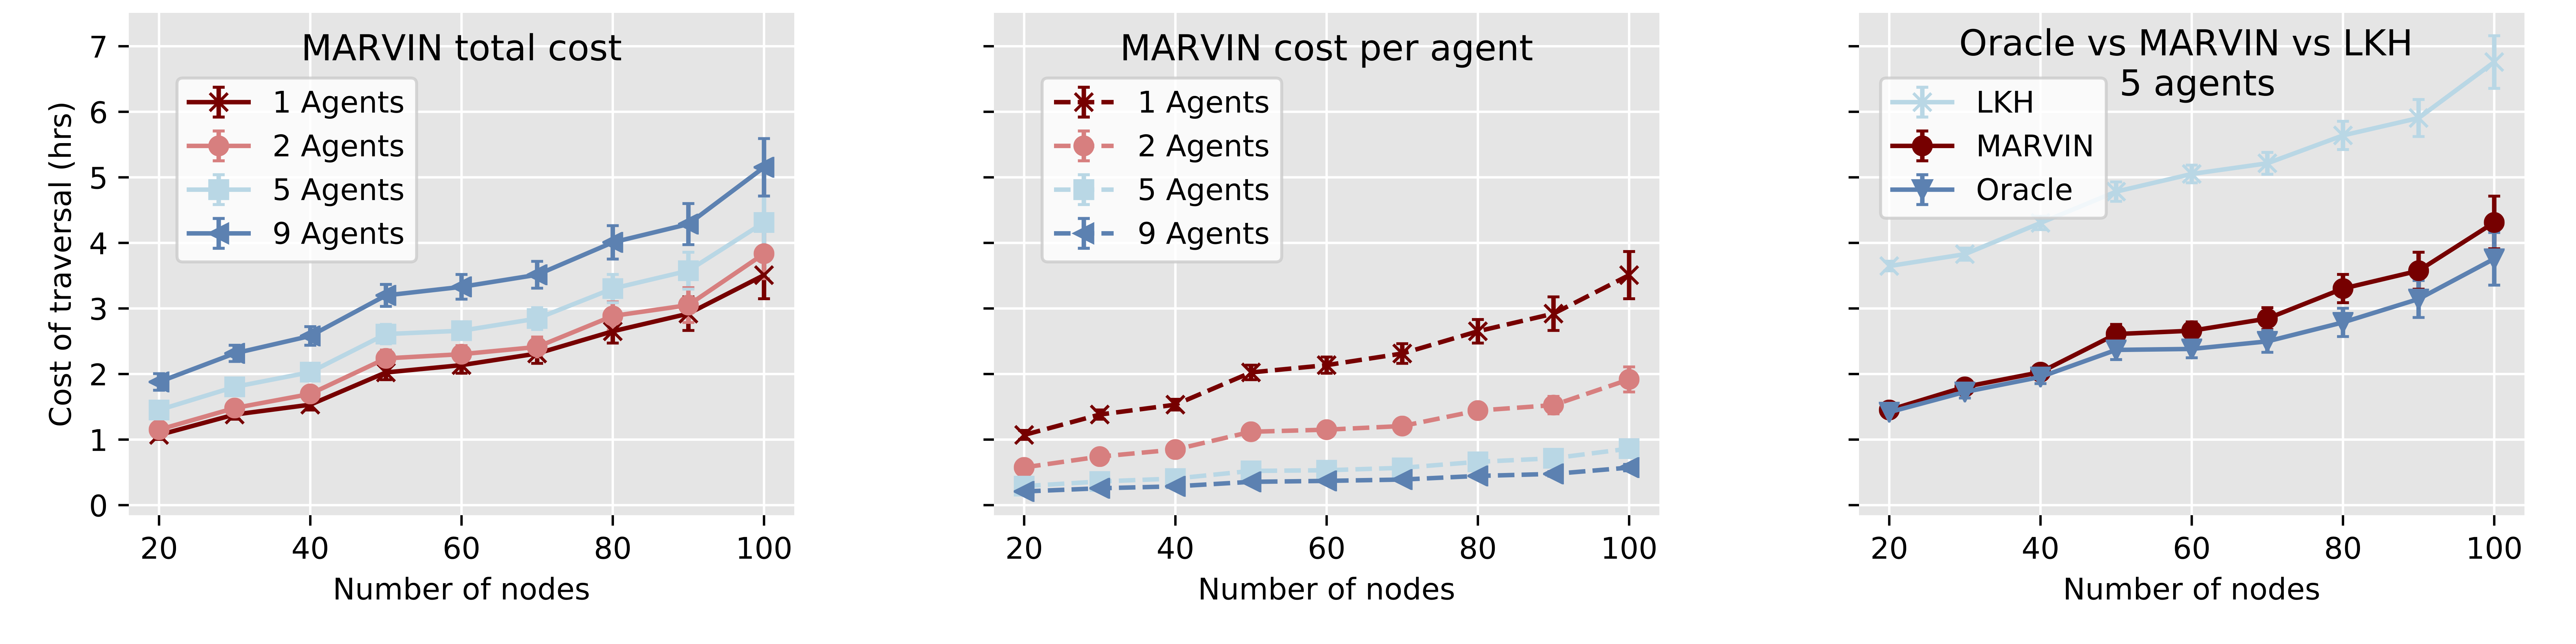
\includegraphics[width=6\textwidth]{figs/scalability.png}
\else
\fi
\centerline{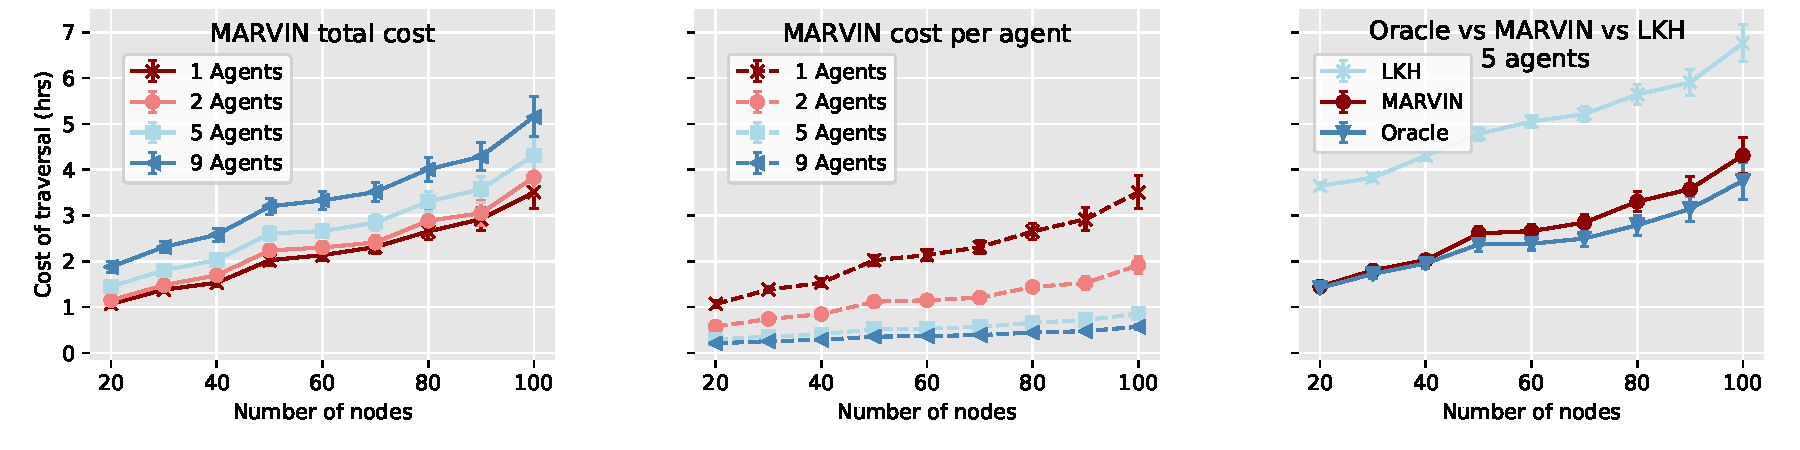
\includegraphics[width=0.95\textwidth,trim={1cm 1cm 1cm 0}]{figs/scalability.pdf}}
\caption{Number of agents performing traversal and corresponding cost of the traversal
(trained using RL)}
\label{fig:scalability}
\end{center}
\vspace{-0.25in}
\end{figure*}
% !TEX root = marvin.tex
  \begin{table*}[t]
  \begin{center}
    \centering
      \resizebox{0.9\textwidth}{!}{%
      \begin{tabular}{c|ccc|ccc|ccc|ccc}
      \toprule
                  & \multicolumn{3}{c}{n = 25, 1 Agent}                & \multicolumn{3}{c}{n = 25, 2 Agents}                   & \multicolumn{3}{c}{n = 50, 2 Agents}            & \multicolumn{3}{c}{n = 100, 5 Agents}              \\
      Method      & Cost          & Gap             & Runtime          & Cost           & Gap             & Runtime             & Cost          & Gap             & Runtime       & Cost          & Gap             & Runtime          \\
      \midrule
      \midrule
      Oracle      & 1.16          & 0.00\%          & 71.3             & 1.28           & 0.00\%          & 438                 & 1.85          & 0.00\%          & 902           & 3.19          & 0.00\%          & 2430             \\
      \midrule
      Random      & 4.45          & 284.9\%         & \textbf{3.15}    & 4.47           & 249.4\%         & \textbf{1.50}       & 8.25          & 345.2\%         & \textbf{1.82} & 18.9          & 492.2\%         & \textbf{2.83}    \\
      Greedy      & 2.12          & 73.7\%          & 3.37             & 2.33           & 81.8\%          & 2.11                & 3.55          & 91.5\%          & 3.57          & 10.4          & 227.0\%         & 22.3             \\
      LKH3        & 1.26          & 8.84\%          & 71.2             & 1.80           & 40.5\%          & 438                 & 2.54          & 37.3\%          & 902           & 6.14          & 92.5\%          & 2430             \\
      \midrule
      GVIN        & 1.37          & 18.8\%          & 52.5             & 1.48           & 15.9\%          & 44.2                & 2.45          & 32.1\%          & 63.4          & 5.41          & 69.6\%          & 48.6             \\
      GAT         & 1.53          & 32.5\%          & 43.0             & 1.56           & 21.6\%          & 29.1                & 2.58          & 39.7\%          & 38.0          & 5.43          & 70.2\%          & 38.2             \\
      AM          & 4.90          & 322.4\%         & 161              & -              & -               & -                   & -             & -               & -             & -             & -               & -                \\
      EAN         & 2.89          & 145.8\%         & 212              & -              & -               & -                   & -             & -               & -             & -             & -               & -                \\
      MARVIN (IL) & 1.37          & 18.0\%          & 62.8             & 1.42           & 11.3\%          & 66.6                & 2.21          & 19.0\%          & 71.5          & \textbf{4.36} & \textbf{36.7\%} & 72.8 \\
      MARVIN (RL) & \textbf{1.25} & \textbf{8.17\%} & 62.8             & \textbf{1.32}  & \textbf{2.87\%} & 56.6                & \textbf{2.12} & \textbf{14.5\%} & 71.4          & 4.62          & 44.9\%          & 72.8 \\
      \bottomrule
      \end{tabular}%
      }
      \caption{Average graph traversal cost on realistic graphs; Time cost in hours; Runtime in milliseconds.}
        \label{tab:1}
        \vspace{-0.2in}
        \end{center}
    \end{table*}


%\subsection{Baselines}
We compare our approach with the following baselines.
\paragraph{Random:} This baseline consists of visiting each node that has not been completely mapped
yet in a random order.

\vspace{-0.1in}
\paragraph{Greedy:} Each agent visits the closest node that still needs to be mapped. It assumes
that the agents are able to communicate which nodes have been fully mapped.

\vspace{-0.1in}
\paragraph{LKH3:} represents the best  performance of the iterative solver given limited information.
We first allow the solver ~\citep{lkh3} to calculate the optimal path for covering each
 node exactly once. Then, the solver calculates a new optimal path over all the remaining
nodes that must be mapped. This is repeated until all nodes have been fully mapped. In essence, the
solver performs VRP traversals until all nodes have been visited the desired number of times.

\vspace{-0.1in}
\paragraph{GVIN:} The Generalized Value Iteration Network~\citep{gvin} uses a GNN to propagate
values on a graph. While the original implementation does not integrate communication between
multiple agents, we enhanced  GVIN with our attention communication module for fair comparison. This
model was trained with imitation learning to achieve  best performance.

\vspace{-0.1in}
\paragraph{GAT:} Graph Attention Networks~\citep{gat} are similar to our method, in that they
exchange information according to attention between two nodes in order to convey complex
information. However, standard GAT architectures do not encode the distance matrix information and
instead assume all edges have an equal weight, limiting their capabilities.
% in a weighted graph domain.
While GATs are not necessarily designed to solve the TSP or VRP problems,  they  remain
one of the state-of-the-art solutions for graph and network encoding.

\vspace{-0.1in}
\paragraph{AM:} The Attention Model~\citep{am}  has been used as a deep learning VRP solver. Since
it has no natural way to encode the information in the adjacency matrix, we add a Graph Convolution Network (GCN) % \raquel{you havent defined GCN}
encoding module at the beginning to perform this encoding and use imitation learning for training. The
modification that the authors suggest for the AM algorithm to allow it to perform a VRP traversal
does not allow for dynamic route adaptation, as is required in our environment. We therefore only
evaluate this method in the single agent scenario.
%\raquel{this is a very odd statement. Where is this modification suggested?}
%\quin{This modification for how to perform VRP is suggested in the original AM paper. They
%compute the VRP solution by repeatedly sending out a single agent and having it return back to
%the starting location instead of trying to coordinate the agents in tandem}

\vspace{-0.1in}
\paragraph{EAN:} Encode-Attend-Navigate~\citep{ean} is a deep learning TSP solver designed very
similarly to AM, but with a slightly different architecture. We enhance it with an additional GCN
module at its beginning to encode the adjacency matrix in the same fashion as with AM. This model
was trained with imitation learning as well.

\vspace{-0.1in}
\paragraph{Oracle:} This is the upper bound performance that an agent could have possibly achieved
if given global information about all the hidden states. This solution is found by providing the
LKH3 solver with details about all the hidden variables, and solving for the optimal plan. We transform
the adjacency matrix by increasing the edge weights of the nodes effected by congestion, and by
duplicating the nodes that will require multiple passes to be fully mapped.

% !TEX root = marvin.tex
\begin{figure*}[t]
\centering
\iflatexml
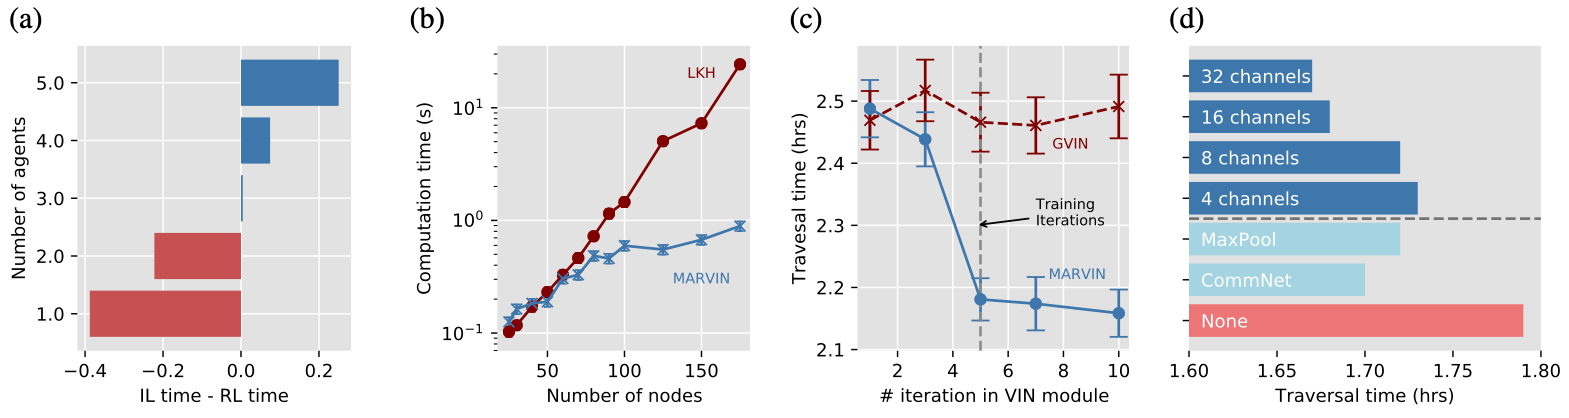
\includegraphics[width=6\textwidth]{figs/figall.png}
\else
\begin{small}
\vspace{-0.1in}
\begin{tabular}{llll}
(a) & (b) & (c) & (d)\\
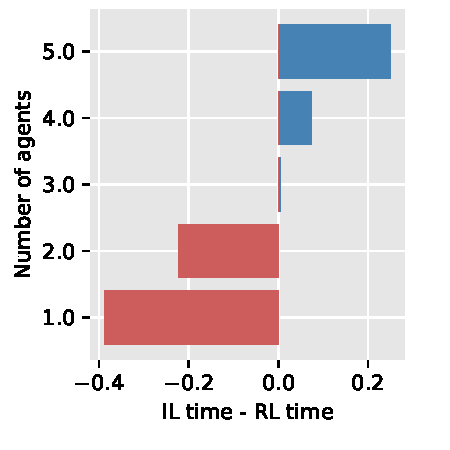
\includegraphics[height=4.1cm,trim={0.2cm 0 0.4cm 0},clip]{figs/diff_cost.pdf} &
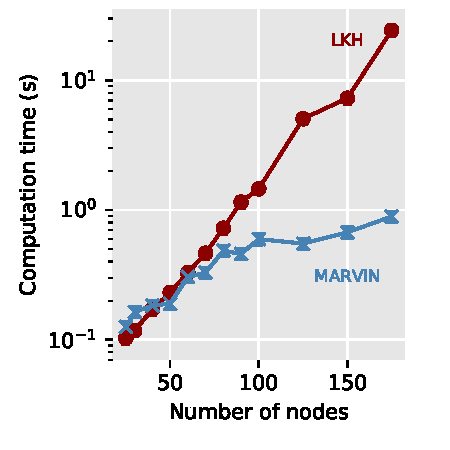
\includegraphics[height=4.1cm,trim={0.2cm 0 0.8cm 0},clip]{figs/runtime.pdf} &
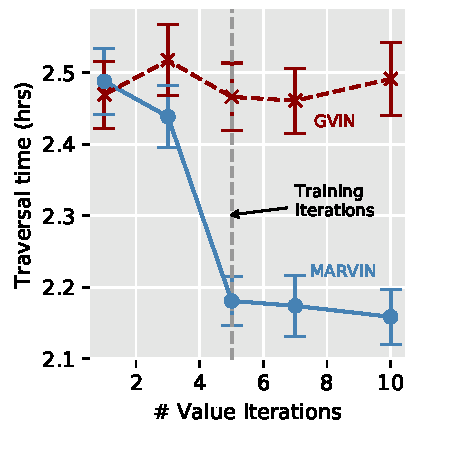
\includegraphics[height=4.1cm,trim={0.2cm 0 0.8cm 0},clip]{figs/iterations} &
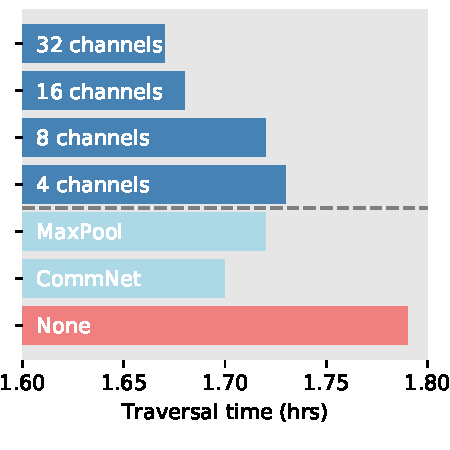
\includegraphics[height=4.1cm,trim={0.0cm 0 0cm 0},clip]{figs/comms}\\
\end{tabular}
\end{small}
\fi
\vspace{-0.1in}
\caption{\textbf{(a) IL vs. RL:} Comparison of imitation learning and reinforcement learning on different number of agents;
\textbf{(b) Runtime:} Comparison MARVIN's runtime to that of the LKH solver;
\textbf{(c) No. iterations in the VIN module:} Evaluation of how the number of value iterations has on performance, and how the number of
    iterations generally scales for other value iteration models (GVIN);
\textbf{(d) Communication module design:} Comparison of our communication protocol to other communication protocol alternatives.
}
\label{fig:all}
\end{figure*}
\subsection{Results}
\vspace{-0.1in}
\paragraph{Comparisons to Baselines:} As shown in Table~\ref{tab:1}, our method has the best
performance across different numbers of agents and graph sizes. Notably, under 25 nodes and two
agents, which is the training setting, our method with RL achieves a total cost that is within 3\%
from that of the oracle. We found our model trained with both reinforcement learning and imitation
learning outperforms all competitor models. Overall, the model shows impressive generalization to
more agents and larger graph size, since we limit the training of the model with two agents and 25
nodes. We also note that deep learning-based solvers that perform well in the more traditional TSP
domain (AM, EAN) are unable to generalize well to our realistic benchmark. Specifically, the low
performance of these deep learning solvers can be attributed to their inability to cope with mapping
failures and nodes requiring multiple passes, which in turn is the result of their architecture
not being structured for this  problem formulation.
% architecture does not account for these realistic challenges, and the potential for revisits of the
% same node.
% \raquel{this last sentence is redundant with the previous one, or?. merge them}

\vspace{-0.1in}
\paragraph{Load distribution:} The cost of performing each traversal is very evenly spread out
amongs all of the agents. The maximum Gini coefficient for two agents observed on our evaluation set
was 0.169, with the mean coefficient being around 0.075.

\vspace{-0.1in}
\paragraph{Scale to number of agents and graph size:}  One
of the primary focuses of our work is to develop a model that scales well with the number of agents
and the size of the graph. Therefore, we evaluated our model's performance on increasingly large
graphs and observed how the performance varied with the number of agents.  As shown in Fig.~\ref{fig:scalability}, 
 the total cost increases marginally when we increase the total number of agents,
indicating good scalability in this respect, and that our method performs much better than the
current state of the art, as is represented by LKH.

% \raquel{we are missing the link to Fig.~\ref{fig:scalability} and talk aobut what we see on it}

We notice that models trained with RL appear to be able to generalize better when dealing with a
larger number of agents, shown in Fig.~\ref{fig:all}A. This could be explained by the fact that
supervised learning tries to exactly mimic the optimal strategy, which may not carry over when
dealing with more agents, and therefore generalizes less effectively.

We also evaluate how a model trained on only toy graphs with 25 nodes compares with a graph trained
only on toy graphs with 100 nodes.
%\raquel{why are you talking about toy graphs?}
%\quin{I did not generate enough realistic graphs that were 100 nodes in size to run on realistic
%graphs so this experiment was performed on the toy graphs to give a general sense of how our model
%is able to be trained on larger environments if needed}
As shown in Fig.~\ref{fig:retrained} ,the 100 node model scales much
better on larger graphs, but that  25 node version of the model is able to perform much closer to
true optimal when acting on smaller graphs.

% !TEX root = marvin.tex

\begin{figure}[t]
\begin{center}
\iflatexml
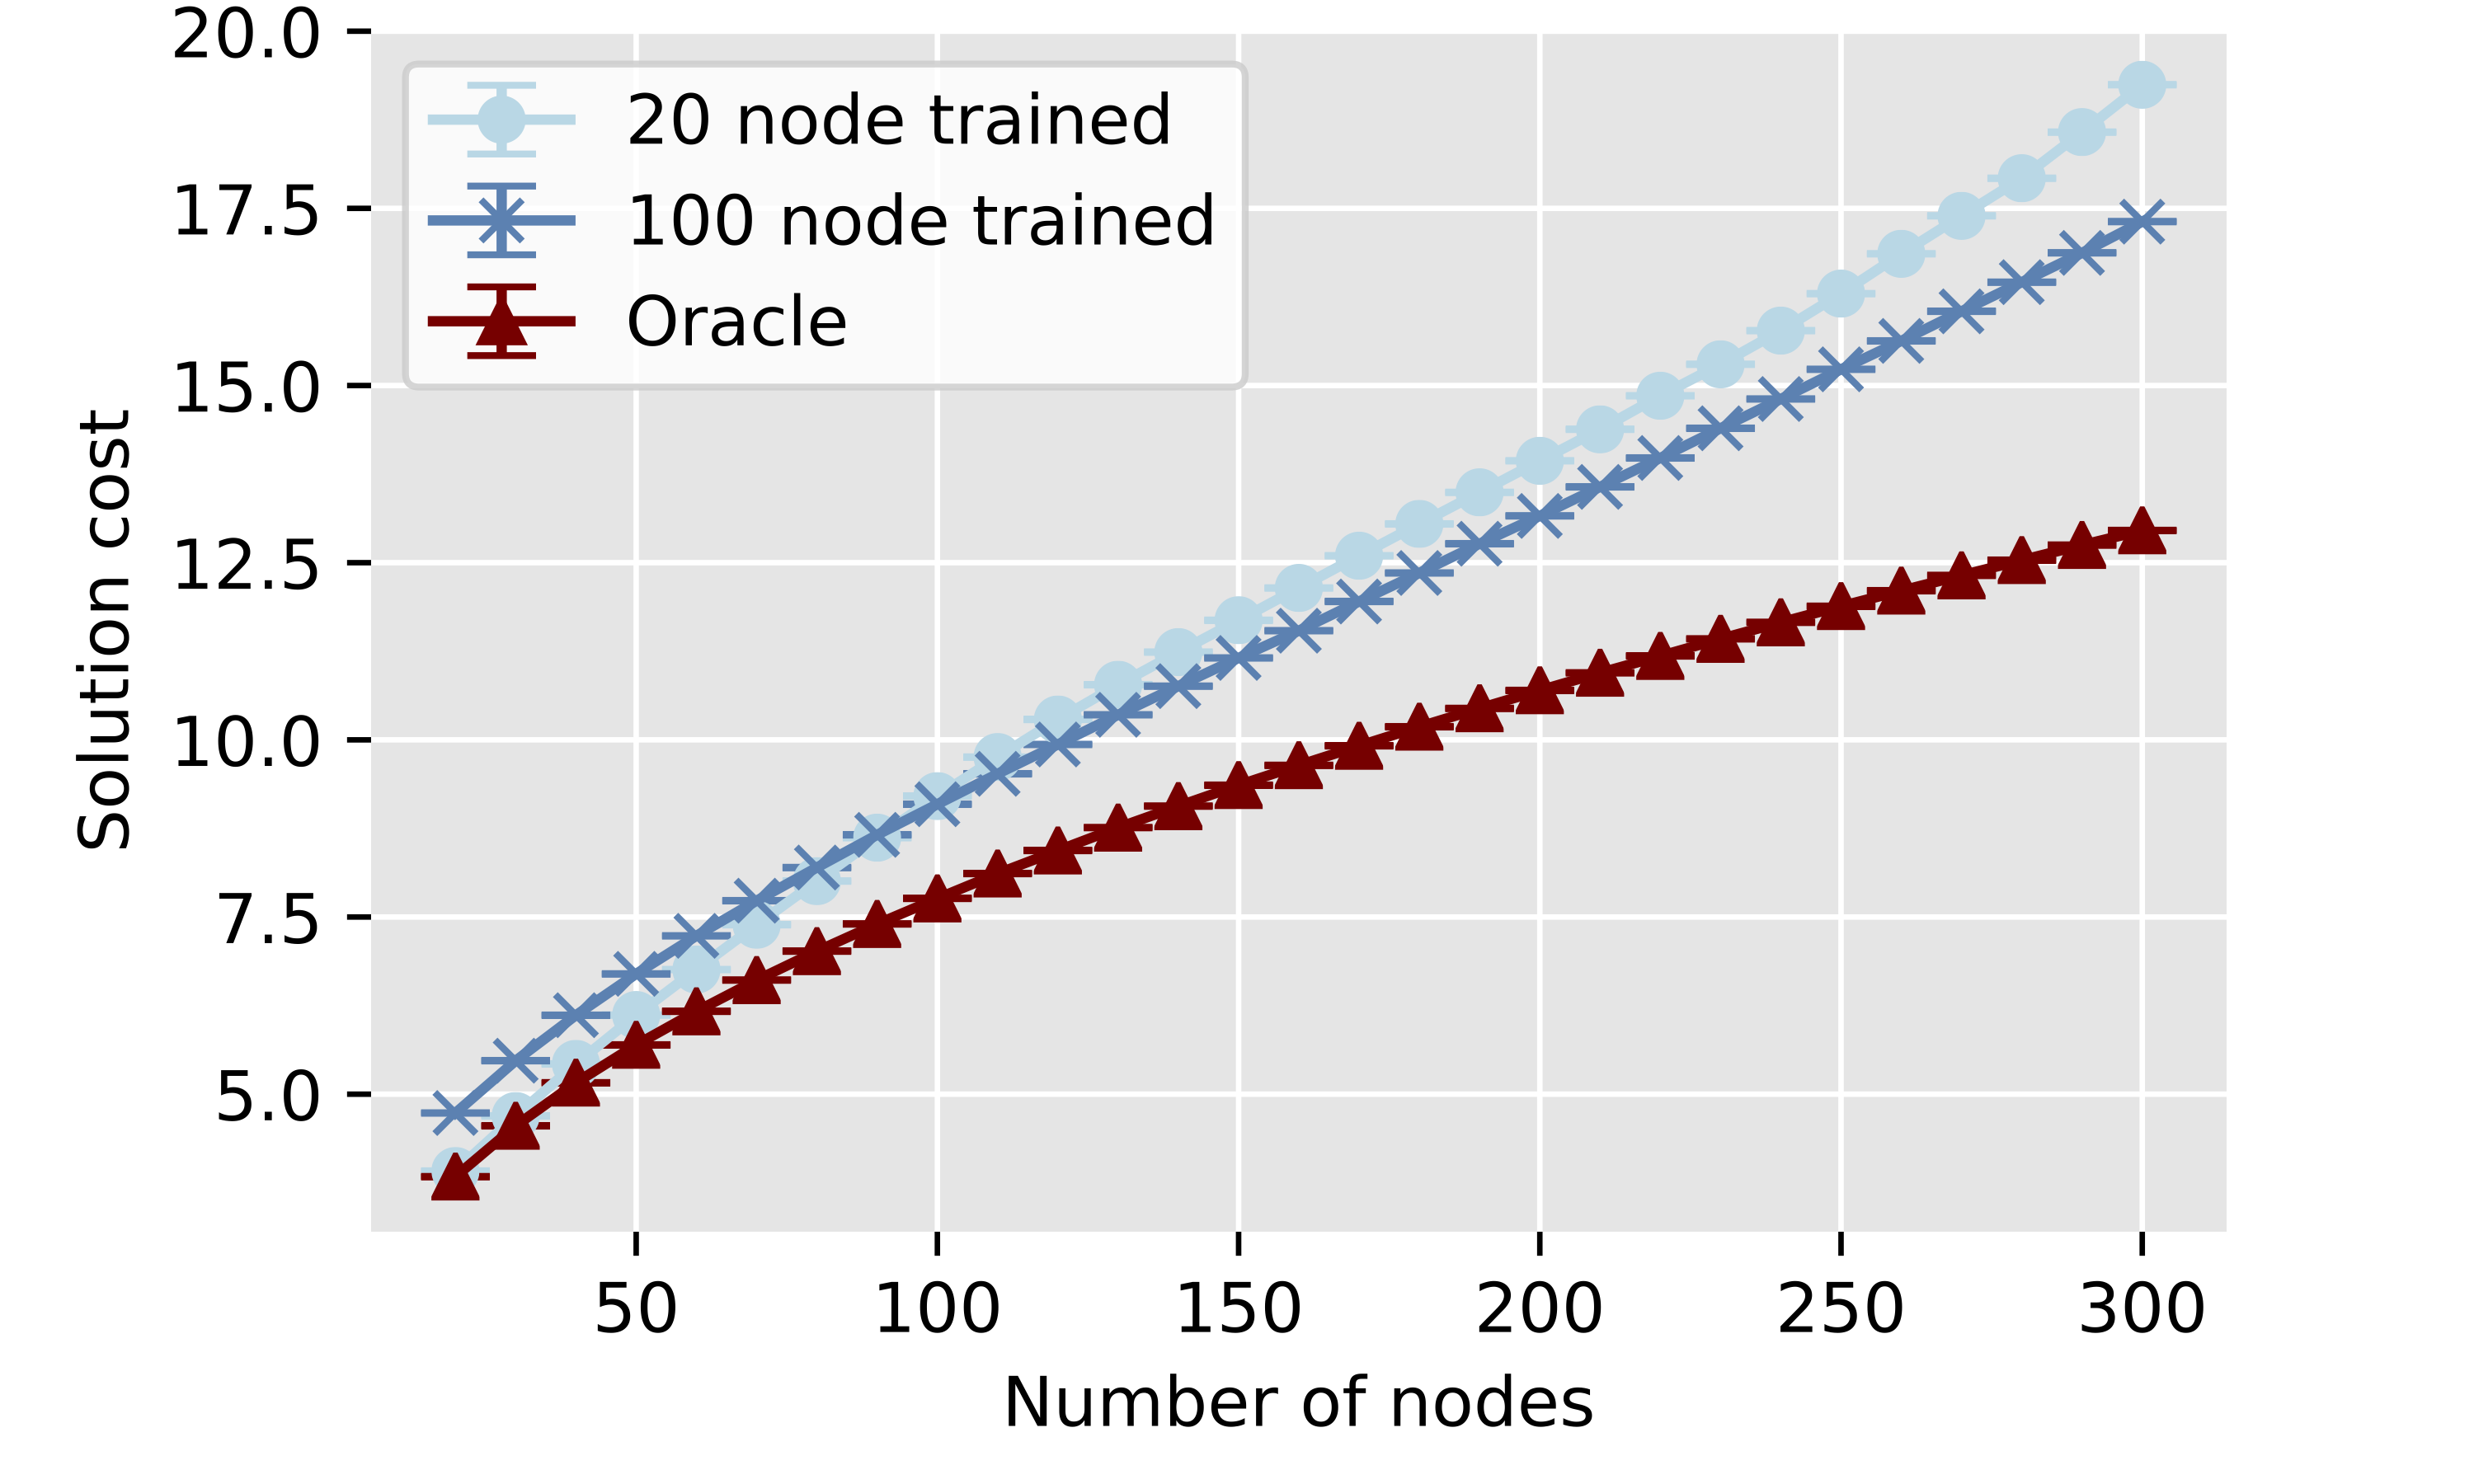
\includegraphics[width=6\columnwidth]{figs/sizes.png}
\else
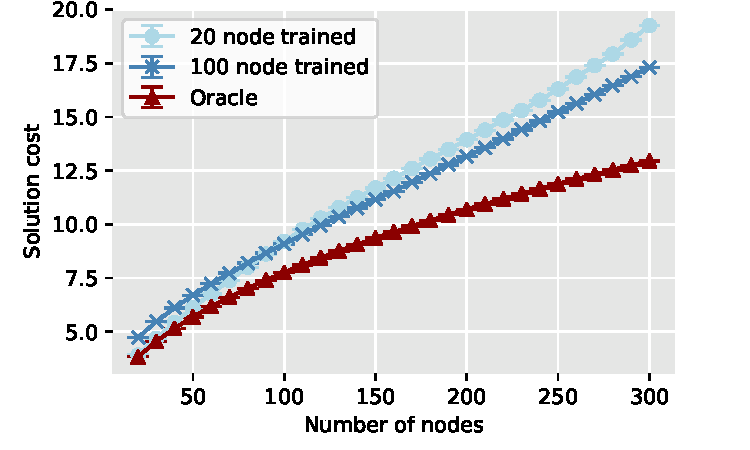
\includegraphics[width=0.94\columnwidth]{figs/sizes.pdf}
\fi
\vspace{-0.2in}
\caption{The average traversal time (hrs) relative to the number of nodes in the graph
for policies trained exclusively on 25 node graphs and 100 node graphs
}
\vspace{-0.25in}
\label{fig:retrained}
\end{center}
\end{figure}

\vspace{-0.1in}
\paragraph{Runtime:} An  advantage that deep learning solutions have over conventional
solvers is their runtime. We compare the average runtime of our model versus that of the LKH3
solver in Fig.~\ref{fig:all}B. Note that our model is significantly faster than LKH3 on large
scale graphs with over 100 nodes.

\vspace{-0.1in}
\paragraph{Robustness to distribution shift:} We also evaluate the generalizability of our model to
different ``multiple pass'' distributions. In order to simulate realistic mapping failures, each
node must be revisited an unknown number of times before we say that it has been completely mapped.
The ``multiple pass'' distributions is the distribution from which these numbers are selected.
% \raquel{explain here what you mean by multiple pass}
Shown in Table~\ref{tab:multipass}, our model has a
consistent performance when we change the distribution at test time, despite being trained
exclusively on the uniform 1-3 distribution.

% !TEX root = marvin.tex
\begin{table}[t]
\begin{center}
\begin{small}
\resizebox{0.9\columnwidth}{!}{%
\begin{tabular}{c|c|ccc}
\toprule
Multi-pass distribution & Oracle & LKH3  & Ours (RL)     & Ours (IL)     \\
\midrule
Uniform 1 - 3           & 1.28   & 1.80  & \textbf{1.32} & 1.42          \\
Uniform 1 - 5           & 1.92   & 3.05  & \textbf{2.11} & 2.20          \\
Uniform 1 - 10          & 3.50   & 5.72  & \textbf{3.82} & 4.24          \\
TruncGaussian 1 - 3     & 1.51   & 2.52  & \textbf{1.75} & 1.79          \\
Either 2 or 4           & 1.72   & 2.49  & \textbf{1.84} & 2.01          \\
Only 3                  & 1.52   & 1.92  & \textbf{1.68} & \textbf{1.68} \\
Exp (mean = 2)          & 1.67   & 3.26  & \textbf{1.73} & 1.84          \\
\bottomrule
\end{tabular}
}
\end{small}
\vspace{-0.1in}
\caption{Model performance on different multi-pass distributions}
\vspace{-0.2in}
\label{tab:multipass}
\end{center}
\end{table}

\vspace{-0.1in}
\paragraph{Number of value iterations:}
In this experiment, we extend the number of iterations in our value iteration module to see if the
module can benefit from longer reasoning. We originally trained our model with 5 iteration, and find
that when we scale the number of iterations up to 10 during evaluation, the performance also further
increases, as is seen in Fig.~\ref{fig:all}C.

% !TEX root = marvin.tex
\begin{table}[t]
\begin{center}
\begin{small}
      \resizebox{0.9\columnwidth}{!}{%
\begin{tabular}{c|cccc}
\toprule
Method                              & Network Size    & Cost            & Gap             & Runtime         \\
\midrule
Concorde (Oracle)                   & -               & 4.22            & 0.00\%          & 40.1            \\
LKH3                                & -               & 4.22            & 0.00\%          & 159             \\
OR Tools                            & -               & 4.27            & 1.11\%          & 15.0            \\
\midrule
Random Insertion                    & -               & 4.44            & 5.12\%          & \textbf{2.31}   \\
Nearest Insertion                   & -               & 4.84            & 14.7\%          & 15.4            \\
Farthest Insertion                  & -               & 4.34            & 2.36\%          & 4.66            \\
Nearest Neighbour                   & -               & 5.02            & 19.0\%          & 14.2            \\
\midrule
AM (SS)                             & 28 MB           & 4.24            & 0.51\%          & 16.3            \\
AM (SS + SP)                        & 28 MB           & 4.23            & 0.13\%          & 552             \\
MARVIN                              & 0.04 MB           & 4.54            & 7.56\%          & 61.7            \\
MARVIN (SS)                         & 0.04 MB           & 4.32            & 2.38\%          & 18.9            \\
MARVIN (SS + SP)                    & 0.04 MB           & \textbf{4.23}   & \textbf{0.10\%} & 1714            \\
\bottomrule
\end{tabular}
}
\end{small}
\caption{Single agent TSP on synthetic graphs of size 25.
We abbreviate methods that make use of \emph{self-starting} with \textbf{SS}
and \emph{sampling} with \textbf{SP}.}
\label{tab:toy}
\end{center}
\vspace{-0.2in}
\end{table}

\vspace{-0.1in}
\paragraph{Toy TSP:} To validate that our model can also solve toy TSP problems and thoroughly be
compared with previous methods under their settings, we run a single-agent TSP benchmark with graphs
of size 25 and uniformly generated vertices in a 1 by 1 square, following \citep{am}. Random,
Nearest, and Farthest insertion, as well as nearest neighbour and AM are all taken from~\cite{am}.
Usually, in our problem setting the agent has no control over where it begins. However, since a
complete TSP tour is independent of its starting position, we also test the effect of letting our
model choose its starting position, which we denote as \emph{self-starting}. We also evaluate how
other conventional tour augmentation techniques affect our model's performance.
\emph{Sampling} takes random samples from the action space of each of the agents and chooses the
one with the lowest overall cost. When augmenting the method with trajectory sampling, we sample
from 1280 model-guided stochastic runs.
%\raquel{why that value? odd}
%\quin{okay to be honest, which I was running this experiment I meant to type in 1028 but I think I accidentally
%typed it in wrong so this ended up being the value I used since I didn't really think it mattered}
As shown in Table~\ref{tab:toy}, we find that even though our model performs worse than the state-of-the-art attention model when we simply take a single greedy trajectory, it is able to outperform it
when both models are augmented with trajectory sampling, getting within 0.10\% of the optimal. It is
also worth noting that our model is 800 times smaller than the best performer in terms of the number
of parameters.

\vspace{-0.1in}
\paragraph{Visualization of large scale mapping:} We also visualize our model navigating a swam of
agents on a large portion of Chicago. Here we perform a large scale autonomous mapping simulation
with a fleet of 20 vehicles on a graph of size 2426 nodes.
% Our visualization will be released very
% soon \mengye{Add blog link}. \raquel{this is very odd, either you have the blog link or you have some figure in the paper}
We generally observe that when compared to other deep learning
solutions, our model results in a much more thorough sweep, where it more rarely has to revisit
previously seen regions. We further observe that models trained with imitation learning  adopt more ``exploratory'' strategies, where
agents split from the main swarm to visit new regions. For more details on the implications of this strategy
please refer to the Appendix
% \raquel{explain why this is not good}

% !TEX root = marvin.tex
\begin{table}[t]
    \begin{center}
    \begin{small}
    \resizebox{0.85\columnwidth}{!}{%
    \begin{tabular}{c|ccc|c}
    \toprule
    Variant                &  Attn. & Dense adj. & LSTM         & Action Acc.    \\
    \midrule
    GVIN                   &             &            &             & 65.4\%          \\
    GAT                    & \checkmark  &            &             & 23.5\%          \\
    No LSTM                & \checkmark  & \checkmark &             & 71.7\%          \\
    Full                   & \checkmark  & \checkmark & \checkmark  & \textbf{75.8\%} \\
    \bottomrule
    \end{tabular}
    }
    \end{small}
    \caption{Action prediction accuracy on different value iteration module designs.
    All models are trained using imitation learning.}
    \vspace{-0.25in}
    \label{tab:accuracy}
    \end{center}
\end{table}
%\subsection{Ablation studies}
\vspace{-0.1in}
\paragraph{Value iteration module:}
We investigated various design choices of the value iteration module, shown in
Table~\ref{tab:accuracy}, where we train different modules using IL and test them in
terms of action prediction accuracy. As shown, GVIN, lacking the dense adjacency matrix and
attention mechanism, is significantly worse than our model, and adding an LSTM further improves the
performance by allowing an extended number of iterations of value reasoning.

\vspace{-0.1in}
\paragraph{Communication module:}
We investigated different potential designs of the communication module,
including CommNet style, MaxPooling, and the number of channels. As shown in Fig.~\ref{fig:all}D, we found that our attention based
modules performs significantly better. Furthermore, the performance is improved with more channels.



